\documentclass[11pt]{article}

\usepackage[margin=1in]{geometry}
\usepackage{graphicx}
\usepackage{booktabs}
\usepackage{amsmath}
\usepackage{amssymb}
\usepackage{hyperref}
\usepackage{xcolor}
\usepackage[export]{adjustbox}
\usepackage{tikz}
\usetikzlibrary{arrows.meta, positioning, calc, fit}

\title{\textbf{ZKLoRA: Efficient Zero-Knowledge Proofs for LoRA Verification}}
\author{ 
\includegraphics[height=8em]{figs/bagel-logo-bw.png} \\
    \textbf{Bidhan Roy, Peter Potash, Marcos Villagra} \\
    Bagel Research Team\footnotemark[1] \\
    \texttt{bidhan@bagel.net, peter@bagel.net, marcos@bagel.net}
}
\date{\today}

\begin{document}

\maketitle

\footnotetext[1]{Bagel is a research lab, making open source AI monetizable.}

\begin{abstract}
    Parameter-efficient fine-tuning (PEFT) techniques, including Low-Rank Adaptation (LoRA), are widely adopted to customize large-scale language models in distributed training environments. A base model user may want to use LoRA weights developed by an external contributor, creating two requirements: the base model user must verify that the LoRA weights are effective when combined with the designated open-source model, and the contributor must protect proprietary parameters until compensation is assured.
    
    We propose \textbf{ZKLoRA}, a zero-knowledge protocol that leverages polynomial commitments, succinct proofs, and advanced cryptographic designs to confirm LoRA–base model compatibility \emph{without} disclosing private LoRA weights. Our evaluations show that verification requires only \textbf{1--2 seconds} per LoRA module for typical large models. This short verification time enables trust-driven collaboration across decentralized infrastructures and contract-based training pipelines, ensuring that the delivered LoRA is valid while preserving the contributor’s intellectual property.
\end{abstract}

%------------------------------------------
% INTRO: emphasize verification challenge & clarify it's per-module
%------------------------------------------
\section{Introduction}
Large Language Models (LLMs) have attained remarkable success \cite{brown2020language, devlin2018bert}, but verifying fine-tuned modifications such as LoRA \cite{hu2021lora} can be difficult when the updated weights must remain private. 
Traditionally, one might re-run an entire forward pass or inspect thousands of parameters to ensure correctness, which is infeasible for massive models. 
\texttt{ZKLoRA} addresses this by generating a zero-knowledge proof of correctness for each LoRA module, guaranteeing that the private LoRA genuinely fits the public base model. 
Crucially, \textbf{the verification stage for each LoRA module} in \texttt{ZKLoRA} remains about 1--2 seconds, even at scales of multi-billion parameter base models. 
This rapid, per-module check allows the Base Model User to efficiently, independently verify the compatibility of the private LoRA parameters.

%------------------------------------------
% 1. PRELIMINARY RESULTS
%------------------------------------------
\section{Preliminary Results}

We benchmarked \texttt{ZKLoRA} across several LLMs and smaller models with different numbers of LoRA modules. 
Our central question is how verification times, as well as settings and proof generation times, grow with \textbf{the number of LoRA modules}, while also considering each LoRA's average parameter size. 
Figure~\ref{fig:verify_vs_numlora} and Table~\ref{tab:settings_proof} detail this trade-off. \footnote{Note that the number of LoRA modules in a given model is not purely a function of the number of layers -- it is also a choice of which weight matrices within each layer is targeted. For example, just targeting one matrix per layer (ie the Query matrix in the Attention Block) will yeild one LoRA per layer. Conversely, targeting the Query, Key, and Value matrices yields three matrices per layer and makes the total number of LoRAs $3 \times num$\_$layers$.}

\begin{figure}[ht]
    \centering
    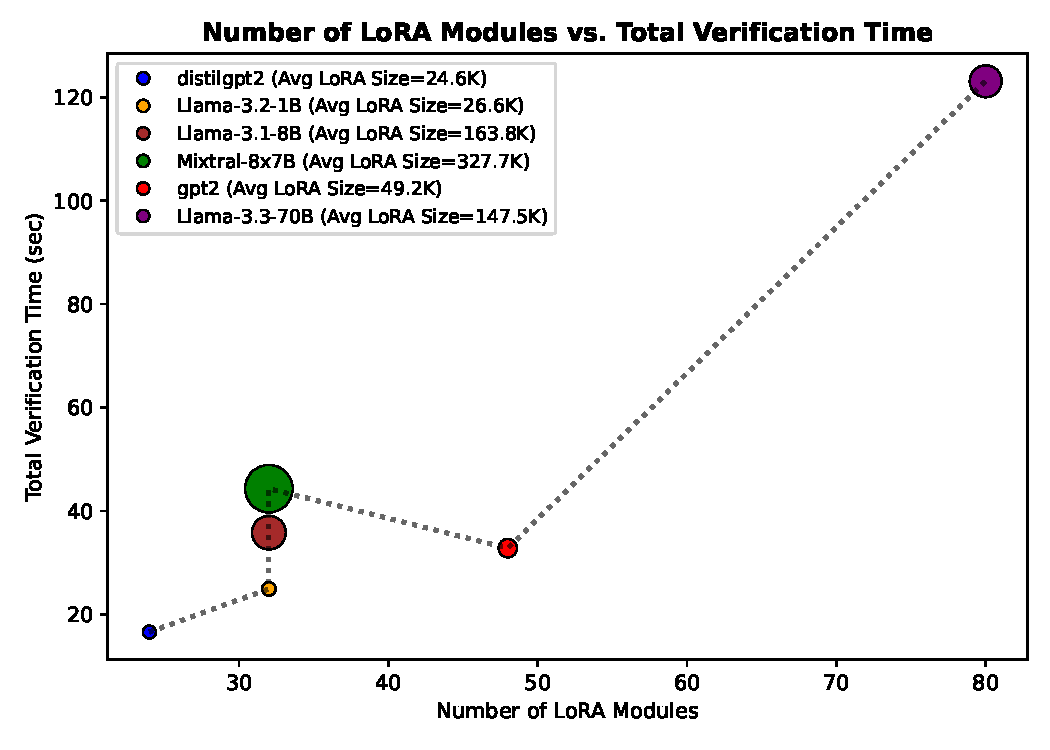
\includegraphics[width=0.9\linewidth]{figs/fig_verify_vs_numlora.pdf}
    \caption{Total verification time (seconds) vs. number of LoRA modules, with dot size reflecting average LoRA size.}
    \label{fig:verify_vs_numlora}
\end{figure}

\begin{table}[h]
\centering
\begin{tabular}{lcccc}
\hline
Base Model & \# of LoRAs & Avg LoRA Size & Avg Settings & Avg Proof \\
\hline
distilgpt2 & 24 & 24576 & 38.0 & 31.6 \\
openai-community/gpt2 & 48 & 49152 & 43.6 & 34.9 \\
meta-llama/Llama-3.2-1B & 32 & 26624 & 37.2 & 31.0 \\
meta-llama/Llama-3.3-70B-Instruct & 80 & 147456 & 54.9 & 46.9 \\
meta-llama/Llama-3.1-8B-Instruct & 32 & 163840 & 57.4 & 47.7 \\
mistralai/Mixtral-8x7B-Instruct-v0.1 & 32 & 327680 & 86.1 & 73.7 \\
\hline
\end{tabular}
\caption{Model benchmark results for Settings and Proof generation time averaged by number of LoRA modules.}\label{tab:settings_proof}
\end{table}

From Figure~\ref{fig:verify_vs_numlora}, we see that models with a higher LoRA count (e.g., 80 modules for a large 70B model) can indeed lead to larger total verification time overall. However, the slope remains modest due to \texttt{ZKLoRA}’s succinct design. For instance, even if each module is verified individually at around 1--2 seconds, verifying 80 modules can be done in just a few minutes, which is still practical for real-world usage.

Table~\ref{tab:settings_proof} similarly shows that \emph{proof generation} and \emph{settings time} scale with the number of LoRA modules, but also depend heavily on each module’s average size (indicated by larger or smaller dot size). These two steps (proof generation on the LoRA contributor’s side and cryptographic circuit setup) can become more expensive, yet remain feasible in decentralized settings or paid contract relationships. The \emph{Base Model User}, meanwhile, benefits from the relatively short verification overhead.

Overall, these plots confirm that \texttt{ZKLoRA} can handle multiple LoRA modules with minimal overhead for verifying correctness, emphasizing the viability of repeated or multi-adapter scenarios in large-scale LLM pipelines.

%------------------------------------------
% 2. Ensuring LoRA–Base Model Compatibility with ZKLoRA
%------------------------------------------
\section{Ensuring LoRA–Base Model Compatibility}

A typical workflow involves:
\begin{enumerate}
    \item \textbf{Base Model User} possessing a large LLM. 
    \item \textbf{LoRA Contributor} having proprietary low-rank adapter weights. 
\end{enumerate}
However, these two parties must confirm the LoRA truly “fits” the base model. Using \texttt{ZKLoRA}, the LoRA Contributor proves the adapter’s compatibility \emph{without} exposing private weights:

\begin{enumerate}
    \item \textbf{Partial Forward Pass.}
    The Base Model User runs the unaltered layers of the LLM, producing partial activations.

    \item \textbf{LoRA Transform + Proof Gen.}
    The LoRA Contributor applies private LoRA forward passes based on partial activations, constructing a zero-knowledge proof to attest correct usage.

    \item \textbf{Verification per LoRA Module (1--2 sec).}
    The user verifies each proof quickly, ensuring the final outputs reflect a valid LoRA for the base model.

    \item \textbf{Evaluate.}
    With trust in the LoRA’s correctness, the user measures performance (e.g. loss).
\end{enumerate}

\iffalse
\begin{figure}[ht]
\centering
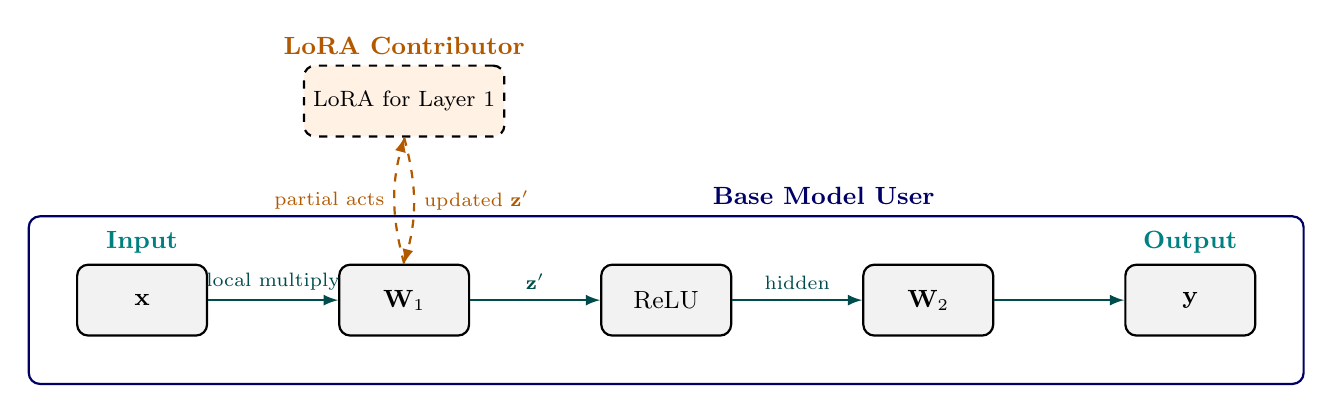
\begin{tikzpicture}[
    font=\small,
    >=latex,
    thick,
    block/.style={
      draw,
      rounded corners,
      align=center,
      minimum width=1.65cm,  % Decreased from 1.8cm to 1.65cm
      minimum height=0.9cm,
      fill=gray!10  % Light gray background for regular blocks
    },
    dashedblock/.style={
      draw,
      dashed,
      rounded corners,
      align=center,
      font=\footnotesize,
      fill=orange!10,  % Light orange background for LoRA block
      minimum width=1.65cm,  % Decreased to match other blocks
      minimum height=0.9cm
    },
    arrow/.style={->, thick},
    node distance=1.65cm  % Decreased from 1.8cm to 1.65cm
]
\node[block, label=above:\textcolor{teal}{\textbf{Input}}] (input) {$\mathbf{x}$};
\node[block, right=1.65cm of input] (W1) {$\mathbf{W}_1$};
\node[dashedblock, above=1.6cm of W1, label=above:\textcolor{orange!70!black}{\textbf{LoRA Contributor}}] (LoRA) {LoRA for Layer 1};
\node[block, right=1.65cm of W1] (act) {ReLU};
\node[block, right=1.65cm of act] (W2) {$\mathbf{W}_2$};
\node[block, label=above:\textcolor{teal}{\textbf{Output}}, right=1.65cm of W2] (output) {$\mathbf{y}$};
\draw[->, teal!60!black] (input) -- node[above, font=\scriptsize]{local multiply} (W1);
\draw[->, dashed, orange!70!black] (W1.north) to[bend left=15] node[left, font=\scriptsize]{partial acts} (LoRA.south);
\draw[->, dashed, orange!70!black] (LoRA.south) to[bend left=15] node[right, font=\scriptsize]{updated $\mathbf{z}'$} (W1.north);
\draw[->, teal!60!black] (W1) -- node[above, font=\scriptsize]{$\mathbf{z}'$} (act);
\draw[->, teal!60!black] (act) -- node[above, font=\scriptsize]{hidden} (W2);
\draw[->, teal!60!black] (W2) -- (output);
\node[draw, rounded corners, thick, color=blue!40!black,
      fit=(input)(W1)(act)(W2)(output),
      label={[font=\small, color=blue!40!black, xshift=2cm]above:\textbf{Base Model User}},
      inner sep=0.6cm
] (baseModelFit) {};
\end{tikzpicture}
\caption{zklora inference flow on a 2-layer neural network where the first layer has private LoRA weights added.}
\label{fig:toy-mlp-lora}
\end{figure}
\fi

\begin{figure}[ht]
\centering
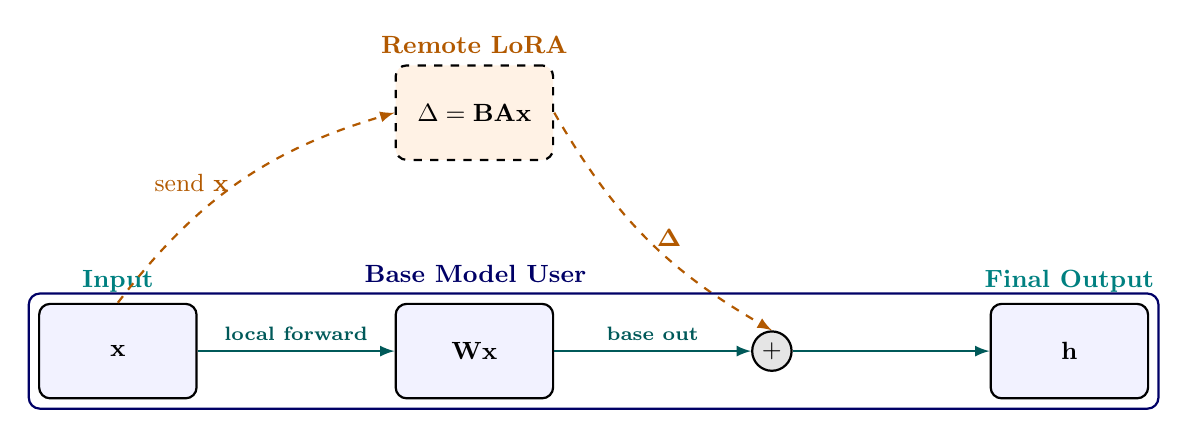
\begin{tikzpicture}[
    font=\small,
    >=latex,
    thick,
    block/.style={
      draw,
      rounded corners,
      align=center,
      minimum width=2cm,
      minimum height=1.2cm,
      fill=blue!5
    },
    dashedblock/.style={
      draw,
      dashed,
      rounded corners,
      align=center,
      fill=orange!10,
      minimum width=2cm,
      minimum height=1.2cm
    },
    sumblock/.style={
      draw,
      circle,
      fill=gray!20,
      inner sep=1pt,
      minimum size=0.5cm
    },
    arrow/.style={->, thick},
    node distance=2.5cm
]

% 1) Input x
\node[block, label=above:\textcolor{teal}{\textbf{Input}}] (xnode) {\(\mathbf{x}\)};

% 2) Local submodule (removed label)
\node[block, right=2.5cm of xnode] (localSub) {\textbf{Wx}};

% 3) Summation or aggregator (removed z label)
\node[sumblock, right=2.5cm of localSub] (sumNode) {\(+\)};

% 4) Final output
\node[block, right=2.5cm of sumNode, 
      label=above:\textcolor{teal}{\textbf{Final Output}}] (finalOut) {%
\(\textbf{h}\)};

% 5) The dashed remote LoRA block
\node[dashedblock, above=1.8cm of localSub, 
      label=above:\textcolor{orange!70!black}{\textbf{Remote LoRA}}] 
(lora) {\(\Delta = \mathbf{BAx}\)};

% ARROWS
% x -> localSub
\draw[->, teal!70!black] (xnode) -- node[above, font=\scriptsize]{\textbf{local forward}} (localSub);

% localSub -> aggregator
\draw[->, teal!70!black] (localSub) -- 
   node[above, font=\scriptsize]{\(\textbf{base out}\)} (sumNode);

% aggregator -> final
\draw[->, teal!70!black] (sumNode) -- (finalOut);

% x -> remote LoRA (increased font size)
\draw[->, dashed, orange!70!black] (xnode.north) to[bend left=18]
   node[left, font=\small]{send \(\mathbf{x}\)} (lora.west);

% remote LoRA -> aggregator (increased font size)
\draw[->, dashed, orange!70!black] (lora.east) to[bend right=15]
   node[right, font=\small]{\(\mathbf{\Delta}\)} (sumNode.north);

% Base Model box with label shifted left
\node[
  draw,
  rounded corners,
  thick,
  color=blue!40!black,
  fit=(xnode)(localSub)(sumNode)(finalOut),
  label={[font=\small, color=blue!40!black, xshift=-1.5cm]above:\textbf{Base Model User}}
] (baseBox) {};

\end{tikzpicture}
\caption{Flow in a Multi-Party Inference scenario between local base model and remote LoRA weights. 
The base model performs a local forward pass, computing \(\mathbf{base\_out} = \mathbf{Wx}\). In parallel, the input \(\mathbf{x}\) is sent to the remote LoRA module, which returns \(\mathbf{\Delta} = \mathbf{BAx}\), where \(\mathbf{B,A}\) are the low-rank finetuned matrices. The final output is \(\mathbf{base\_out} + \mathbf{\Delta}\).}
\label{fig:remote-lora-flow}
\end{figure}





%------------------------------------------
% 3. HOW WE GENERATE THE ZERO-KNOWLEDGE PROOF
%------------------------------------------
\section{Zero-Knowledge Proof Generation}

\texttt{ZKLoRA} compiles an ONNX model (with LoRA included) into a constraint circuit. The user’s partial activations feed the circuit as inputs:

\paragraph{(1) Circuit Compilation.} 
We parse the LoRA-augmented layers, producing a cryptographic circuit capturing each parameter operation. 

\paragraph{(2) Key Setup.} 
A settings file, proving key, and verification key are generated. A structured reference string (SRS) may also be needed.

\paragraph{(3) Witness Creation.}
The LoRA Contributor runs the partial activations through the circuit, tracking all wire values in a “witness.” 

\paragraph{(4) Proof.}
Using the witness plus proving key, the LoRA Contributor constructs a proof. 

\paragraph{(5) Verification per Module.}
Each LoRA module’s proof is tested with the verification key, taking \textbf{1--2 seconds}. This minimal overhead is \texttt{ZKLoRA}’s main advantage for frequent or large-scale checks.

%------------------------------------------
% 4. RELATED WORK
%------------------------------------------
\section{Related Work}

\subsection{Low-Rank Adaptation (LoRA)}
Low-Rank Adaptation (LoRA) \cite{hu2021lora} is a technique for parameter-efficient fine-tuning of large language models (LLMs) that injects small, low-rank adapter matrices into specific layers of a pre-trained model. By isolating the fine-tuning process to these low-rank components, LoRA drastically reduces memory overhead compared to full-model fine-tuning. This design choice is especially appealing for massive LLMs where training or even storing all parameters can be prohibitive \cite{ding2022delta}.

Beyond the clear advantage of reduced storage, LoRA also facilitates swapping multiple domain-specific adapters into a single base model, making it straightforward to maintain separate skill sets without instantiating an entire new copy of the model. These adapters can target specialized tasks (e.g., medical or legal text) with minimal overhead, driving LoRA’s widespread adoption. Yet verifying that a proprietary LoRA truly aligns with a base model (without revealing the adapter) remains problematic—precisely the gap \texttt{ZKLoRA} fills.

\subsection{Incrementally Verifiable Computation}
In a decentralized world, trust is a resource that is hard to achieve. In decentralized computation, we need to make sure the computations are both done and done correctly. In a seminal paper by Valiant (2008) \cite{valiant2008incrementally}, it was shown that proofs of knowledge can be used to assert the correct execution of general computations. That is, if $M$ is a machine that runs for $t$ steps producing a sequence of configurations $c_0,c_1,\dots,c_t$, then there exist an efficient and effective way to produce a computationally sound proof for the computation $c_0  \xrightarrow{t} c_t$. This idea is referred to as Incrementally Verifiable Computation or IVC.

The main goal of IVC is to produce compact, updatable proofs of correctness for a sequence of computations, so that each new step can be verified on its own while building on the guarantees of previous steps. This technique significantly reduces the verification overhead for long or evolving computations, which is invaluable in scenarios like decentralized networks, outsourced computation, and any application requiring frequent correctness checks.

Kumar et al. (2021) \cite{kothapalli2022nova} introduced the proof system NOVA and the idea of recursive proofs, which are proofs that can ``prove the correctness of other proofs.'' Recursive proof composition is key to IVC where each proof attests to the correctness of both a step’s output and the validity of the previous step’s proof.

HyperNova \cite{kothapalli2024hypernova} is a novel recursive argument system optimized for customizable constraint systems (CCS) that generalizes and improves upon prior approaches like Nova. It achieves efficiency through a folding scheme where the prover’s cryptographic costs are minimized and achieves zero-knowledge without relying on zkSNARKs. An IVC system allows the construction of proofs in zero-knowledge where the proofs reveal no information about the underlying computation or its inputs beyond the validity of the claim \cite{valiant2008incrementally}.

%------------------------------------------
% 5. CONCLUSION
%------------------------------------------
\section{Conclusion}

\texttt{ZKLoRA} provides a fast, robust mechanism to ensure that private LoRA modules remain consistent with a large base model. Our evaluations indicate that each LoRA module’s correctness can be verified in less than 2 seconds, even for multi-billion-parameter LLMs. This efficiency bridges the gap between privacy-preserving LoRA development and practical, real-time validation in large-scale deployments. In terms of future work, the most relevant and immediate work would be adding polynomial commitments of the base model's activations (those that are sent as input to the LoRA contributor). This would take us one step closer to providing end-to-end verifiability of inference computation for LoRA-finetuned models.  Other avenues of expansion could be integrating multi-contributor LoRAs, advanced zero-knowledge proofs for further performance gains, or partial data-privacy frameworks to shield user inputs as well as LoRA parameters. 

\bibliographystyle{plain}
\bibliography{references}

\end{document}
